\documentclass[tikz,border=4pt]{standalone}
\usepackage{tikz}
\begin{document}
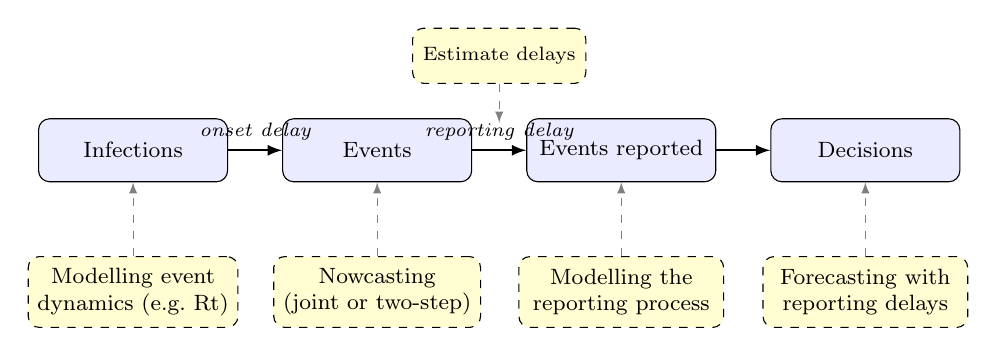
\begin{tikzpicture}[
  every node/.style={align=center, font=\footnotesize},
  stage/.style={draw, rounded corners, minimum height=8mm,
                minimum width=24mm, fill=blue!8},
  method/.style={draw, dashed, rounded corners, minimum height=9mm,
                 minimum width=26mm, fill=yellow!18},
  delaybox/.style={draw, dashed, rounded corners, minimum height=7mm,
                   minimum width=22mm, fill=yellow!18, font=\scriptsize},
  arr/.style={->, thick, >=latex},
  marr/.style={->, dashed, gray, >=latex}
]
  \node[stage] (a) at (0,0) {Infections};
  \node[stage] (b) at (3.1,0) {Events};
  \node[stage] (c) at (6.2,0) {Events reported};
  \node[stage] (d) at (9.3,0) {Decisions};

  \draw[arr] (a) -- node[above, font=\scriptsize\itshape]{onset delay} (b);
  \draw[arr] (b) -- node[above, font=\scriptsize\itshape]{reporting delay} (c);
  \draw[arr] (c) -- (d);

  \node[delaybox] (md) at (4.65,1.2) {Estimate delays};
  \draw[marr] (md) -- (4.65,0.35);

  \node[method] (m1) at (0,-1.8) {Modelling event\\dynamics (e.g.\ Rt)};
  \node[method] (m2) at (3.1,-1.8) {Nowcasting\\(joint or two-step)};
  \node[method] (m3) at (6.2,-1.8) {Modelling the\\reporting process};
  \node[method] (m4) at (9.3,-1.8) {Forecasting with\\reporting delays};

  \draw[marr] (m1) -- (a);
  \draw[marr] (m2) -- (b);
  \draw[marr] (m3) -- (c);
  \draw[marr] (m4) -- (d);
\end{tikzpicture}
\end{document}
